\begin{minipage}{0.75\linewidth}
\begin{figure}[h]
    \centering
    \begin{adjustbox}{max width=1.0\linewidth, keepaspectratio}
        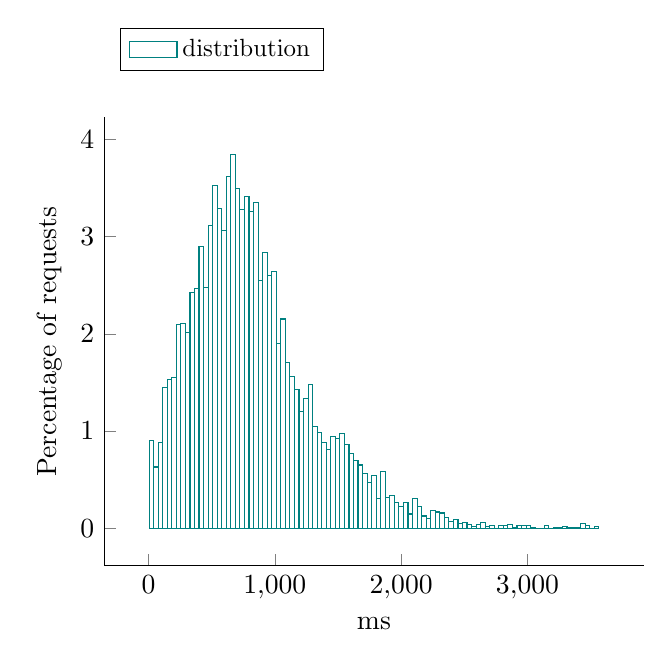
\begin{tikzpicture}
            \begin{axis}[ylabel = Percentage of requests, 
xlabel = ms, 
legend style = {nodes={scale=0.9, transform shape}, at={(0.03,1.2)}, anchor=north west, draw=black, fill=white, align=left, legend columns=3},
area style, mark size = 0pt,
 cycle list name = exotic,
  axis lines* = left]
		\addplot +[ybar interval] coordinates {
			 (5, 0.902982)
			 (40.95, 0.629987)
			 (76.9, 0.881982)
			 (112.85, 1.44897)
			 (148.8, 1.53297)
			 (184.75, 1.55397)
			 (220.7, 2.09996)
			 (256.65, 2.11046)
			 (292.6, 2.01596)
			 (328.55, 2.42545)
			 (364.5, 2.46745)
			 (400.45, 2.89794)
			 (436.4, 2.47795)
			 (472.35, 3.11844)
			 (508.3, 3.52793)
			 (544.25, 3.28643)
			 (580.2, 3.06594)
			 (616.15, 3.62243)
			 (652.1, 3.84292)
			 (688.05, 3.49643)
			 (724, 3.27593)
			 (759.95, 3.41243)
			 (795.9, 3.25493)
			 (831.85, 3.34943)
			 (867.8, 2.55145)
			 (903.75, 2.83494)
			 (939.7, 2.60395)
			 (975.65, 2.64595)
			 (1011.6, 1.90046)
			 (1047.55, 2.15246)
			 (1083.5, 1.70097)
			 (1119.45, 1.56447)
			 (1155.4, 1.42797)
			 (1191.35, 1.19698)
			 (1227.3, 1.33347)
			 (1263.25, 1.48047)
			 (1299.2, 1.04998)
			 (1335.15, 0.98698)
			 (1371.1, 0.881982)
			 (1407.05, 0.808484)
			 (1443, 0.944981)
			 (1478.95, 0.923982)
			 (1514.9, 0.97648)
			 (1550.85, 0.860983)
			 (1586.8, 0.766485)
			 (1622.75, 0.692986)
			 (1658.7, 0.650987)
			 (1694.65, 0.566989)
			 (1730.6, 0.472491)
			 (1766.55, 0.545989)
			 (1802.5, 0.304494)
			 (1838.45, 0.587988)
			 (1874.4, 0.314994)
			 (1910.35, 0.335993)
			 (1946.3, 0.262495)
			 (1982.25, 0.220496)
			 (2018.2, 0.262495)
			 (2054.15, 0.146997)
			 (2090.1, 0.304494)
			 (2126.05, 0.220496)
			 (2162, 0.125997)
			 (2197.95, 0.104998)
			 (2233.9, 0.178496)
			 (2269.85, 0.167997)
			 (2305.8, 0.157497)
			 (2341.75, 0.115498)
			 (2377.7, 0.0734985)
			 (2413.65, 0.0944981)
			 (2449.6, 0.052499)
			 (2485.55, 0.0629987)
			 (2521.5, 0.0419992)
			 (2557.45, 0.0209996)
			 (2593.4, 0.0419992)
			 (2629.35, 0.0629987)
			 (2665.3, 0.0209996)
			 (2701.25, 0.0314994)
			 (2737.2, 0)
			 (2773.15, 0.0314994)
			 (2809.1, 0.0314994)
			 (2845.05, 0.0419992)
			 (2881, 0.0104998)
			 (2916.95, 0.0314994)
			 (2952.9, 0.0314994)
			 (2988.85, 0.0314994)
			 (3024.8, 0.0104998)
			 (3060.75, 0)
			 (3096.7, 0)
			 (3132.65, 0.0314994)
			 (3168.6, 0)
			 (3204.55, 0.0104998)
			 (3240.5, 0.0104998)
			 (3276.45, 0.0209996)
			 (3312.4, 0.0104998)
			 (3348.35, 0.0104998)
			 (3384.3, 0.0104998)
			 (3420.25, 0.052499)
			 (3456.2, 0.0314994)
			 (3492.15, 0)
			 (3528.1, 0.0209996)
			 (3564.05, 0.0209996)
		};
\addlegendentry{distribution};
           \end{axis}
      \end{tikzpicture}
  \end{adjustbox}
  \caption{Response time distribution - req = ReadUser-2}
\end{figure}
\end{minipage}\hfill\begin{minipage}{0.18\linewidth}
\begin{table}[h]
\begin{tabular}{|cc|}
\hline
\textbf{} & \textbf{ms}\\ \hline
 \Xhline{0.005\arrayrulewidth}
min & 5\\
 \Xhline{0.005\arrayrulewidth}
max & 3600\\
 \Xhline{0.005\arrayrulewidth}
mean & 837\\
 \Xhline{0.005\arrayrulewidth}
std & 502\\
\hline
\hline
 \Xhline{0.005\arrayrulewidth}
25th & 492\\
 \Xhline{0.005\arrayrulewidth}
50th & 752\\
 \Xhline{0.005\arrayrulewidth}
75th & 1076\\
 \Xhline{0.005\arrayrulewidth}
80th & 1189\\
 \Xhline{0.005\arrayrulewidth}
85th & 1330\\
 \Xhline{0.005\arrayrulewidth}
90th & 1530\\
 \Xhline{0.005\arrayrulewidth}
95th & 1792\\
 \Xhline{0.005\arrayrulewidth}
99th & 2371\\
\hline
\end{tabular}
\caption{Response time}
\end{table}
\end{minipage}\hfill